%%=============================================================================
%% Methodologie
%%=============================================================================

\chapter{Methodologie}
\label{ch:methodologie}

%% TODO: Hoe ben je te werk gegaan? Verdeel je onderzoek in grote fasen, en
%% licht in elke fase toe welke stappen je gevolgd hebt. Verantwoord waarom je
%% op deze manier te werk gegaan bent. Je moet kunnen aantonen dat je de best
%% mogelijke manier toegepast hebt om een antwoord te vinden op de
%% onderzoeksvraag.
Dit hoofdstuk beschrijft hoe men het best te werk kan gaan in de opzet van een \textit{eenvoudig, kleinschalig blockchain gebaseerd stemsysteem}. Het doel is om een praktische en complete handleiding te vormen, hoofdzakelijk gericht op ontwikkelaars die niet vertrouwd zijn met het ontwikkelen van Ethereum Dapps, noch met het ontwikkelen van cryptografische stemsystemen. 

Gezien de vrij technische aard van deze handleiding wordt er van uit gegaan dat de lezer een algemene voorkennis heeft op het vlak van programmatie en enigszins bekend is met Javascript. Kennis van de taal Solidity wordt niet verondersteld. Tenslotte wordt er veronderstelt dat de lezer over een basis kennis Engels beschikt, daar de volledige code-basis in die taal geschreven is. 

De  verschillende implementatie keuzes die hier wordt gemaakt gebeuren op basis van verschillende concepten en technieken die werden toegelicht in het vorig hoofdstuk. Zo wordt er bijvoorbeeld gekozen voor het Ethereum platform als ontwikkelomgeving op basis van sectie \ref{sec:ethereum-en-smart-contracts} en voor de cryptografie van het zelf-tellende stemprotocol OVNP \autocite{McCorry2017} uit sectie \ref{sec:OVNP}.

In dit hoofdstuk trachten we ook verder antwoord te bieden op enkele van onderzoeksvragen van deze scriptie, metname: 
\begin{itemize}
	\item \textit{wat de praktikaliteit van een blockchain gebaseerd stemsysteem is}
	\item \textit{hoe haalbaar is een blockchain gebaseerd stemsysteem} 
	\item \textit{of er sprake van een onoverkomelijk schaalbaarheidsprobleem}
\end{itemize}

\section{Benodigdheden}
\label{sec:benodigdheden}
	De volgende zaken dienen geïnstalleerd te worden voor men van start kan gaan met het implementeren van een gedecentraliseerde Ethereum blockchain applicatie:
	\begin{itemize}
		\item{Node.js}
		\item{npm}
		\item{Truffle}
		\item{Ganache}
		\item{Metamask}
	\end{itemize}
	Daarnaast heeft men ook nodig:
	\begin{itemize}
		\item{Een IDE code-editor naar keuze met syntax ondersteuning voor Solidity}
		\item{Google Chrome}
	\end{itemize}
	\subsection{ node en npm}
	Node.js is een populaire Runtime-omgeving waarmee Javascript op ieder platform uitgevoerd kan worden, zonder dat daar een browser voor nodig is. Npm is een pakketbeheerder voor Javascript code. Npm zit standaard in Node.js en is `s werelds grootste softwareregister. Open source-ontwikkelaars wereldwijd gebruiken het om pakketten te delen, veel organisaties gebruiken npm om ook hun privéontwikkeling te beheren (\ref{fig:nodejs}).\footnote{Verkregen en vertaald van https://docs.npmjs.com/about-npm/}
	
	Eenmaal node\footnote{node met npm is verkrijgbaar via https://nodejs.org} en npm\footnote{npm is ook apart verkrijgbaar via https://www.npmjs.com/get-npm} geïnstalleerd zijn, verifieert men de installatie via het console-commando: 
	\lstset{language=bash}
	\begin{lstlisting}[numbers=none]
	> node -v
	\end{lstlisting}Bij correcte installatie geeft dit de huidige node versie terug, bijvoorbeeld \textit{v10.15.1}. 
	
	\begin{figure}
		
\includegraphics[width=\linewidth/2]{img/nodejs.png}
		
\includegraphics[width=\linewidth/2]{img/npm.png}
		\caption{De Node.js en npm logo's}
		\label{fig:nodejs}
	\end{figure}
	
	\subsection{Truffle}
	Truffle is een ontwikkelomgeving, testframework en asset pipline, gericht op het versoepelen van het Ethereum ontwikkelproces. Het bevat ook verschillende code-templates die als basis kunnen worden gebruikt om gedecentraliseerde applicaties te ontwikkelen.
	
	Truffle kan eenvoudig geïnstalleerd worden via npm (mits dit  voorgeïnstalleerd is) met het console-commando:
	 \lstset{language=bash}
	\begin{lstlisting}[numbers=none]
	> npm install truffle
	\end{lstlisting}
	\subsection{Ganache}
	Ganache\footnote{Ganache is verkrijgbaar via https://www.trufflesuite.com/ganache} is een applicatie die ontwikkelaars in staat stelt om een private Ethereum-blockchain op te zetten. We gebruiken deze blockchain gedurende de volledige ontwikkelperiode. Op deze manier kan men kosteloos smart-contracts ontwikkelen en testen, als men direct op de Ethereum hoofdketen ontwikkelt is er  immers aan iedere transactie  een kost verbonden. 
	
	Ganache biedt ons  niet enkel een lokale blockchain, het biedt ons ook 10 Ethereum accounts om te gebruiken tijdens het ontwikkelen. Deze accounts hebben adressen die corresponderen met adressen op de lokale Ethereum-blockchain. Elke account is vooraf geladen met 100 nep-ether.
	
	Figuur \ref{fig:ganache-blockchain}: Eenmaal Ganache geïnstalleerd is, open we de applicatie. Door het kiezen van de optie \textit{quickstart} zetten we onmiddellijk een lokale blockchain op. 
	
	\begin{figure}
		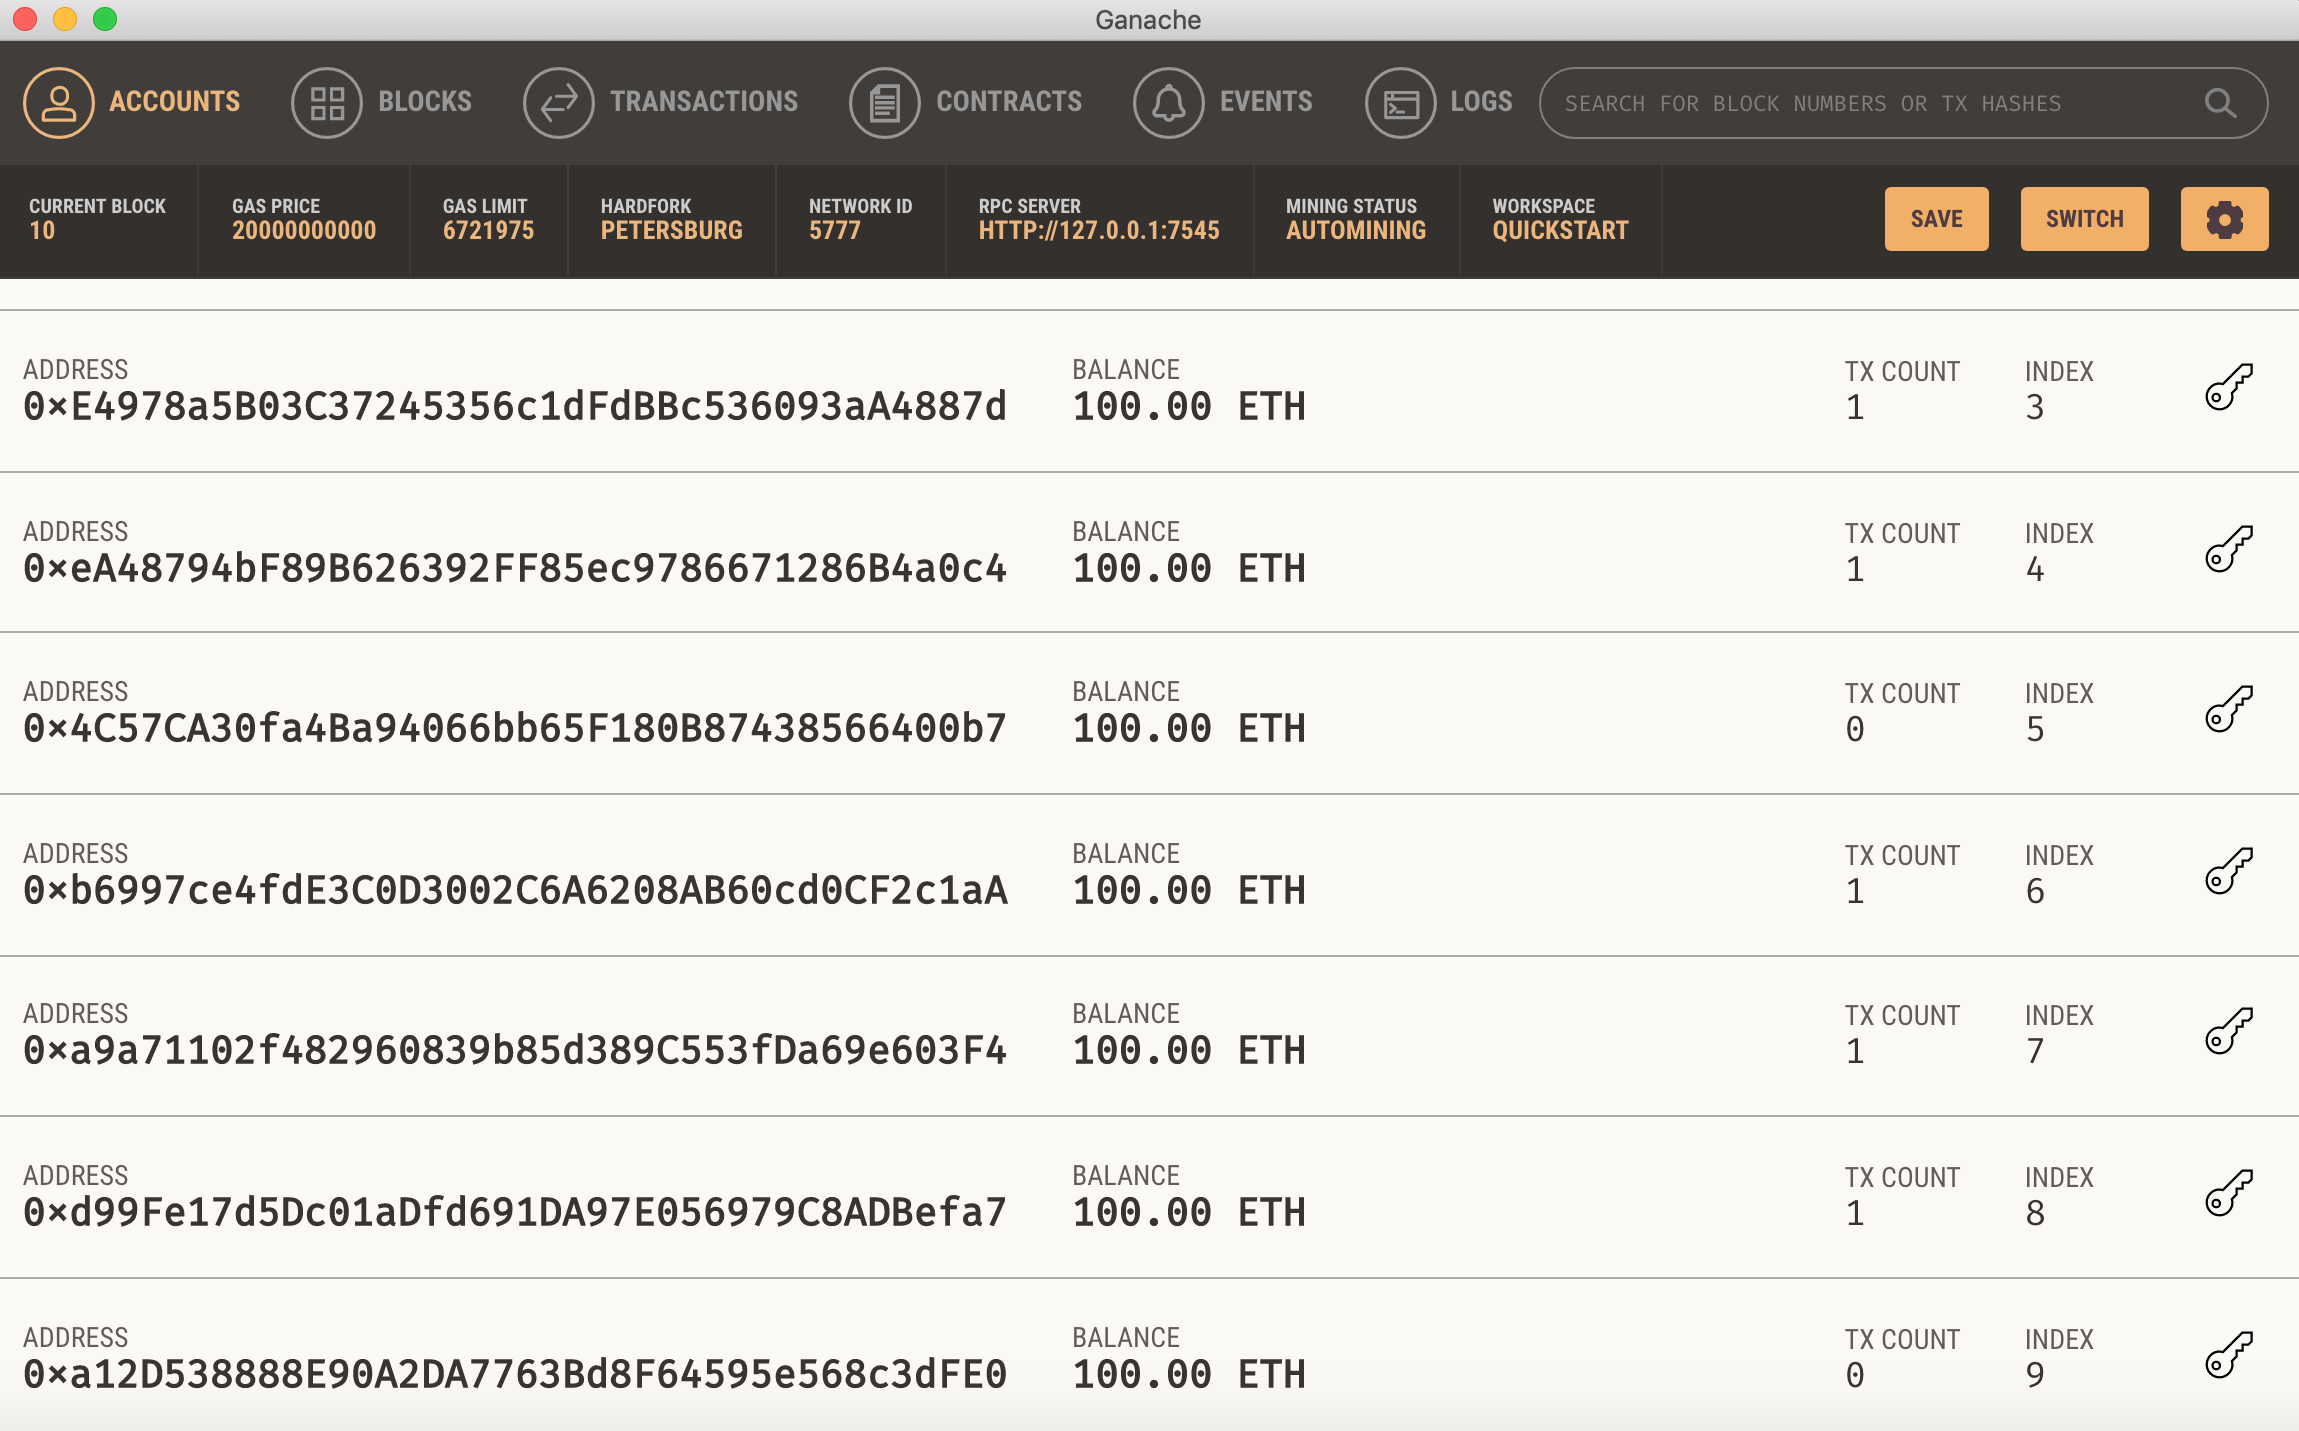
\includegraphics[width=\linewidth]{img/ganache-blockchain.png}
		\caption{Een Lokale blockchain opgezet via Ganache}
		\label{fig:ganache-blockchain}
	\end{figure}
	
	
	\subsection{Metamask}
	Metamask\footnote{Metamask is verkrijgbaar via https://metamask.io of via https://chrome.google.com/webstore} is een Ethereum wallet plugin voor Google Chrome die gebruikers toelaat om transacties van Ethereum dApps uit te voeren in de browser, zonder zelf een node moeten zijn in het netwerk. Door Metamask te installeren hoeft men met andere woorden de volledige blockchain dus niet meer te downloaden. 
	
	Voor deze implementatie is Metamask van cruciaal belang gezien het verantwoordelijk is voor de verificatie van Ethereum accounts. Daarnaast is het ook een zeer handige tool wanneer we onze implementatie in de browser willen testen, het laat ons toe om zeer snel tussen verschillende accounts te verspringen.
	
	Eenmaal de plugin geïnstalleerd is dient men een paswoord te creëren, daarnaast krijgt men ook een fallback sleutel
	
	\begin{figure}
		
\includegraphics[width=\linewidth]{img/metamask-truffle-ganache.png}
		\caption{Truffle, Metamask en Ganache logo's}
		\label{fig:metamask-truffle-ganache}
	\end{figure}
	\newpage
\section{Implementatie Smart Contracts}
	Eenmaal al de verschillende tools en plugins uit sectie \ref{sec:benodigdheden} geïnstalleerd zijn kan men aan het ontwikkelen van smart-contracts beginnen. In de volgende subsecties volgt de implementatie van een blockchain gebaseerd stemsysteem op basis van smart-contracts. We beginnen met een simpele implementatie die niet self-tallying is. In een latere sectie zullen we de nodige cryptografie toevoegen om een systeem gelijkaardig aan het Open Network Protocol van  \textcite{McCorry2017} te bekomen.
	\subsection{Opzet Truffle}
	Voor we beginnen met het ontwikkelen van onze smart-contracts moeten we eerst een ontwikkelomgeving opzetten. Voor een vlotte start maken we gebruik van één van de template projecten beschikbaar via Truffle. 
	
	Na te navigeren naar een gewenste directory, gebruikt men het console commando: 
	 \lstset{language=bash}
	\begin{lstlisting}[numbers=none]
	> truffle unbox pet-shop
	\end{lstlisting}
	
	Dit creëert een nieuw project in de huidige directory, we openen het in een code-editor (Bijvoorbeeld VS-code). Figuur \ref{fig:truffle-template} toont de structuur van de genereerde Truffle template. Het project bevat momenteel zowel een back-end gedeelte (smart-contract) als een front-end (een javascript project). 
	
	In deze handleiding zullen we, met het principe van herbruikbaarheid in gedachten, de code opsplitsen in aparte front- en back-end projecten, de folder en inhoud onder \textit{\slash src}, als ook de afbeeldingen \textit{box-img-lg.png} en \textit{box-img-sm.png} mogen dus uit dit project verwijderd worden.
	
	Het project kan nu als start-template worden gebruikt voor onze implementatie. Voor we van start gaan met implementeren van een smart-contract bekijken we kort de reeds aanwezige code.
	
	\begin{figure}
		\centering
		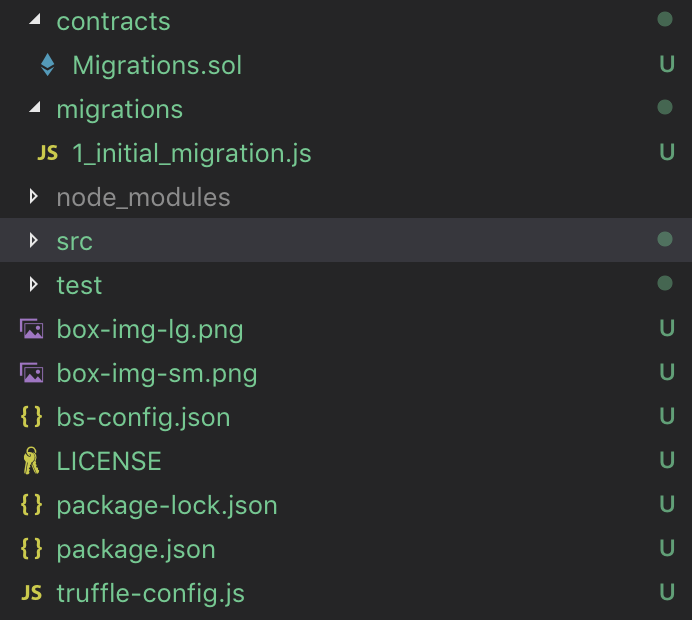
\includegraphics[width=\linewidth/2]{img/truffle-template.png}
		\caption{De structuur van een Ethereum Truffle project}
		\label{fig:truffle-template}
	\end{figure}
	
	\subsection{Migrations}
	De voornaamste bestanden reeds aanwezig in onze template zijn \textit{contracts\slash Migrations.sol} en \textit{migrations\slash 1\_initial\_migration.js}.
	Migrations zijn Javascript-bestanden die  ons helpen bij het deployen van contracten op het Ethereum-netwerk. Deze bestanden worden voornamelijk gebruikt voor het organiseren van de volgorde van deployments en worden geschreven in de veronderstelling dat behoeften hiertoe  in de loop van het ontwikkelingsproces  zullen veranderen. Naarmate een project evolueert, maakt men dus nieuwe migratiescripts om nieuwe code op correcte wijze op de blockchain te krijgen. 
	
	\subsection{Implementatie smart-contract: basis structuur }
	We beginnen met het aanmaken van een nieuw smart-contract bestand op de locatie \textit{contracts\slash Election.sol}. Om een simpel stemsysteem te implementeren in een smart-contract hebben we de volgende zaken nodig:
	\begin{itemize}
		\item een lijst van de `opties' waarop gestemd kan worden
		\item een lijst van de accounts die gestemd hebben
		\item per optie de hoeveelheid stemmen
	\end{itemize}
	We baseren ons hiervoor op implementatie die wordt gegeven door \textcite{McCubin2019}.\footnote{Zie ook https://github.com/dappuniversity/election}
	
	We beginnen met het declareren van de Solidity versie:
	\lstset{language=JavaScriptSolidity} 
	\begin{lstlisting}[numbers=none]
	pragma solidity ^0.5.8;
	\end{lstlisting}
	\lstset{language=JavaScriptSolidity} 

	Vervolgens starten we met het definiëren we van ons smart-contract \textit{Election} :
	\begin{lstlisting}[numbers=none]	
	contract Election {
		constructor () public {
		}
	}
	\end{lstlisting}
	
	Omdat we een lijst van de `opties' willen hebben en ook per optie willen bijhouden hoeveel stemmen er voor zijn, maken we een custom type dat we \textit{Candidate} noemen. 
	
	Onze verkiezing hoeft niet per sé om het verkiezen van een persoon te gaan, het is simpelweg handig om over opties te denken in termen van een `kandidaten'. 
	
	Iedere optie is een kandidaat die een id, een `naam' (de optie tekst) en het aantal voorkeursstemmen heeft. 
	
	In Solidity definiëren we een custom type in de vorm van een \textit{struct}:
	
	\begin{lstlisting}[numbers=none]	
	struct Candidate {
		uint id;
		string name;
		uint votes;
	}
	\end{lstlisting}
	
	We breiden \textit{Election} nu ook uit met volgende attributen:
	
	\begin{lstlisting}[numbers=none]
	//Fetch the candidates	
	mapping(uint => Candidate) public candidates;
	// Store accounts that have voted
	mapping(address => bool) private voters;
	// Read candidate
	uint public candidatesCounter;
	\end{lstlisting}
	
	Het \textit{mapping} keyword in Solidity duidt een hashTable aan, gelijkaardig aan HashMaps in andere programmeertalen. In Solidity is er niet echt een alternatieve datastructuur voor verzamelingen.  Mapping laat ons ook toe om te zoeken op basis van een key. In het geval van  \textit{candiates} mappen we de `kandidaten' op basis van hun id. De id's zijn numeriek en incrementeel. We houden het totaal aantal kandidaten bij in het attribuut `candidatesCounter' zodat we niet onnodig in de mapping moeten zoeken, maar exact weten wat de id's zijn.
	
	In het geval van het attribuut \textit{voters} mappen we de adressen van alle kiezers op een booleaanse-waarde. Willen we weten of een kiezer al een stem heeft uitgebracht, dan kunnen we dit via het \textit{voters} attribuut eenvoudig te weten komen. 
	
	Nu we de basis attributen hebben om een stemsysteem te implementeren moeten we een methode toevoegen aan ons smart-contract `Election' die ons instaat stelt om Candidaten toe te voegen:
	
	\begin{lstlisting}[numbers=none]
	function addCadidate(string memory _name) private {
		candidatesCounter++;
		candidates[candidatesCounter] = Candidate(candidatesCounter,_name,0);
	}
	\end{lstlisting}
	Merk op dat parameter in de bovenstaande functie gemarkeerd is met het Solidity `memory'  keyword. Dit duidt aan dat deze parameter niet in de blockchain dient opgeslagen te worden, de tegenhanger van dit keyword is `storage'.
	
	Voorlopig zullen we onze opties `hardcoden' in de constructor functie, we kiezen voor een implementatie met simpele binaire ja/nee vragen:
	
	\begin{lstlisting}[numbers=none]
	constructor () public {
		addCadidate("Yes");
		addCadidate("No");
	}
	\end{lstlisting}
	
	Nu we opties hebben toegevoegd waarop gestemd kan worden rest ons enkel nog het implementeren van een stem functie. 
	
	\begin{lstlisting}[numbers=none]
	function hasVoted() public view returns (bool ok) {
		return voters[msg.sender];
	}
	\end{lstlisting}
	
	Merk op dat hier gebruik gemaakt wordt van het Solidity \textit{view} keyword, dit duidt aan dat de betreffende functie geen aanpassingen zal maken aan het contract.
	
	\begin{lstlisting}[numbers=none]
	function vote(uint _candidateId) public {
		if(!hasVoted()) {
			// Record voter has voted
			voters[msg.sender] = true;
			// Update candidate vote count
			candidates[_candidateId].votes++;
		}
	}
	\end{lstlisting}
	
	Gezien we wensen dat gebruikers niet meermaals malen een stem kunnen uitbrengen, controleren we bij iedere kiezer of deze al gestemd heeft. We doen dit aan de hand van het \textit{voters} attribuut. Indien de gebruiker nog niet gestemd heeft, stellen we dit in via hetzelfde attribuut. Kiezers die hun stem hebben uitgebracht mappen dus op true waarde, alle andere kiezers zitten nog niet in de mapping, en leveren dus de default waarde false op. Tenslotte verhogen we het aantal stemmen met 1 voor de gekozen optie, deze vinden we door in het \textit{candidates} attribuut te zoeken met de parameter \_candidateId.
	
		\lstset{language=JavaScriptSolidity} 
	\begin{lstlisting}[frame=single] 
	pragma solidity ^0.5.8;
	
	contract Election {
		// Store candidate
		struct Candidate {
			uint id;
			string name;
			uint votes;
		}
		//Fetch the candidates
		mapping(uint => Candidate) public candidates;
		// Read candidate
		uint public candidatesCounter;
		// Constructor
		constructor () public {
			addCadidate("Yes");
			addCadidate("No");
		}
	
		function addCadidate(string memory _name) private {
			candidatesCounter++;
			candidates[candidatesCounter] = 
			Candidate(candidatesCounter,_name,0);
		}
	
		function hasVoted() public view returns (bool ok) {
			return voters[msg.sender];
		}
	
		function vote(uint _candidateId) public {
			if(!hasVoted()) {
				// Record voter has voted
				voters[msg.sender] = true;
				// Update candidate vote count
				candidates[_candidateId].votes++;
			}
		}
	}
	\end{lstlisting}
	
	\subsection{Belang van testen}
	Bij het ontwikkelen van dApps speelt testen nog meer een cruciale rol  dan het bij de traditionele software ontwikkeling doet. Vermits het deployen van contracts op de blockchain verbonden is aan een gas prijs, is het bijzonder onwenselijk dat er bugs in de code sluipen die ervoor kunnen zorgen dat we moeten herdeployen. Functies die bugs bevatten en onverwacht gedrag vertonen kunnen erg kostelijk zijn voor gebruikers door de extra verwerkings-kosten die ze vergen. Doordat alles dat in de blockchain wordt bewaard immutable is betekent het herdeployen van een smart-contract eigenlijk dat het huidige contract wordt vervangen door een nieuwe kopie. Zowel de state als het adres van het oude contract gaan hierbij verloren. Dat is niet alleen bijzonder onpraktisch, het is ook brekend voor iedere front-end applicatie die aan de dApp verbonden is. 
	
	Door smart-contracts grondig te testen kunnen we dergelijke situaties vermijden.
	
	Er zijn verschillende methoden die men kan toepassen om een smart-contract te testen, standaard is om ze te schrijven in Solidity. Voor dit voorbeeld zullen we echter gebruik maken van Javascript. Via Truffle kunnen we met behulp van Javascript de  interacties van gebruikers met onze smart-contracts gemakkelijk simuleren. Truffle bevat immers standaard Mocha\footnote{Apart verkrijgbaar via https://mochajs.org} (testframework) en Chai Assertion Library\footnote{Apart verkrijgbaar via https://www.chaijs.com}. Deze twee tools stellen ons instaat om onze smartcontracts te importeren binnenin Javascript-testen. 
	
	
	 \lstset{language=JavaScriptSolidity} 
	 \begin{lstlisting}
	 var Election = artifacts.require("./Election.sol");
	 	
	 contract("Election", function(accounts){
		var electionInstance;
		 
		it("Initializes two candidates", function() {
		 	return Election.deployed().then(function(instance){
		 		return instance.candidatesCounter();
		 	}).then(function(count){
		 		assert.equal(count,2);
		 	});
	 	});
	 	
		it("Initializes yes and no", function() {
	 		return Election.deployed().then(function(instance){
	 			electionInstance = instance;
	 			return electionInstance.candidates(1);
	 		}).then(function(candidate){
				assert.equal(
			 	candidate[0],1,"has the correct id: 1"
			 	);
				assert.equal(
				 	candidate[1],"Yes","has the correct value: `Yes'"
				);
				assert.equal(
				 	candidate[2],0,"has the correct amount of votes: 0"
				);
				return electionInstance.candidates(2);
	 		}).then(function(candidate){
				assert.equal(
					candidate[0],2,"has the correct id: 2"
				);
				assert.equal(
					candidate[1],"No","has the correct value: `No'"
				);
				assert.equal(
					candidate[2],0,"has the correct amount of votes: 0"
				);
	 		}); // End function
	 	}); // End it()
	}); // End contract
	\end{lstlisting}
	








